\chapter{Análisis de grandes conjuntos de datos} \cite{BIGD}
En EDA como se ha tratado en el tema anterior se pueden usar distintas herramientas para generar hipótesis que sean de interés utilizando las técnicas que ya se han visto como PCA, PLS, score plots, MEDA, etc.
\bigskip

En concreto los score plots son las técnicas que mejor muestran los patrones que se pueden dar en las observaciones. En este tema se explicará una versión de los mismos orientada a problemas con un número de observaciones ilimitadas o muy grandes. Esta técnica se conoce como “Compressed Score Plots” (CSPs).
\bigskip

También se va a comentar la parte de MEDA-Toolbox que se encarga del tratamiento de Big Data y el resto de los métodos de visualización visto en el capítulo anterior.
\bigskip

Los métodos \textbf{BigData} de la toolbox son capaces de lidiar con conjuntos de datos enormes y con flujos de información constantes a altas velocidades manteniendo las capacidades de visualización vistas anteriormente, en tiempos de análisis similares a los problemas de menor tamaño.
\bigskip

\section{¿Qué es Big Data?}
Las nuevas tecnologías facilitan el flujo de información entre distintos sistemas con capacidades de generación de datos inconmensurables, esta gran cantidad de datos es el llamado Big Data.  En campos como la medicina, la química, la física y en el caso que nos ocupa de las redes de computadores, se llegan a generar tantos datos que hay que inventar nuevas técnicas de análisis de los mismos ya que con las clásicas no se puede abordar su análisis.
\bigskip

La definición de Big Data se puede dar con las llamadas “4 uves”:

\begin{itemize}
	\item \textbf{Variedad:}Los datos son formados por distintas fuentes, con distinta naturaleza y estructura.
	
	\item \textbf{Veracidad:}La búsqueda de información relevante en grandes conjuntos de datos es un trabajo complicado y la relación entre señal-ruido en Big Data es baja, por lo que se necesitan técnicas capaces de encontrar patrones de utilidad en la práctica.
	
	\item \textbf{Volumen:}La cantidad de información que se maneja es muy alta.
	
	\item \textbf{Velocidad:}En problemas de Big Data es normal tener grandes flujos constantes de información necesitando ser analizada, por ello la velocidad con la que se procesan los mismos ha de ser alta para resolver los problemas sin que se acumulen más muestras de lo necesario.
	
\end{itemize}


\section{Limitaciones de los Score Plots para grandes conjuntos de datos}

\begin{figure}[H]
\centering
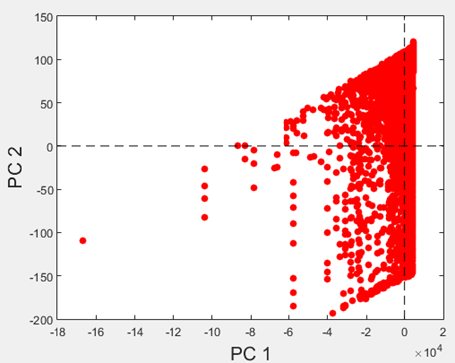
\includegraphics[width=0.9\textwidth]{imagenes/figuras/3_1.png}
\caption{Ejemplo de score plot con BIG DATA.}
\end{figure}

Cuando se utiliza EDA para grandes conjuntos de datos con millones de observaciones que a su vez contienen millones de variables se deben tener en cuenta consideraciones especiales ya que sería imposible dar una representación gráfica comprensible mediante Score plots. Por ello los modelos de proyección de EDA pueden ayudar a reducir el problema pero no lo suficiente para hacer un análisis correcto de lo que sucede.
\bigskip

Como se puede ver en la figura 3.1 en el gráfico es casi imposible establecer patrones o hacerse una idea de las tendencias dentro de un conjunto tan grande de observaciones que emborronan la imagen limitando su utilidad.
\bigskip

Teniendo en cuenta que para el ejemplo de la figura 3.1 se ha utilizado un fichero de datos con 9998 observaciones con 122 variables cada una, y a la hora de analizar Big Data se suelen utilizar varios ficheros de igual o mayor tamaño de forma simultánea, el lector se puede hacer una idea del tamaño del problema a tratar y de como Score plot no es capaz de asimilarlo.

\bigskip
Para solucionar este problema se tiene CSP.

\bigskip

\section{Compressed Score Plots} \cite{CAILS}

El problema de la visualización de Big Data en Score Plots se resuelve mediante técnicas de “clustering”, agrupando observaciones relacionadas mediante gamas de color diferentes para cada cluster, de esta manera se pueden identificar nubes relacionadas a simple vista. 
\bigskip

El criterio que se utiliza para hacer estas agrupaciones es necesario para la creación del cluster, normalmente el más utilizado es el de la distancia. La más popular es la distancia euclídea aunque también se utiliza la distancia de Mahalanobis cuando la diferencia en escala y la correlación de las variables no son despreciables. De forma general la distancia cuadrática se expresa como:
\bigskip

$d_K(x_i-x_j)=\parallel x_i-x_j\parallel_K=((x_i-x_j)^T K^{-1} (x_i-x_j ))^{1/2}$

\bigskip

Donde K es la matriz identidad M-dimensional cuando se utiliza la distancia euclídea y la matriz de covarianza de las variables originales de M en el caso de la distancia Mahalanobis.La inversión de K puede ocasionar problemas al utilizar la distancia de  Mahalanobis. Para evitar dichos problemas se puede restringir dicha inversión a un sub-espacio de proyección como el de PCA o PLS. Dicha inversa de K se calcula:
\bigskip

\begin{itemize}
	\item \textbf{En PCA:} $P*K_{PCA}^{-1}*P^T$
	
	\item \textbf{En PLS:} $P*K_{PLS}^{-1}*P^T$
\end{itemize}

\bigskip

\subsection{Métodos de agrupamiento}
Los métodos de “clustering” o métodos de agrupamiento para Compressed Score Plots, a partir de ahora CSP, no son tarea fácil ya que en el proceso no se pueden destruir datos de interés ni introducir valores inservibles dentro de la distribución de datos. Las técnicas más eficientes para agrupar grandes conjuntos de datos son:
\bigskip

\begin{itemize}
	\item Búsqueda eficiente de vecinos cercanos   
	
	\item Resumen de datos.
	
	\item Computación distribuida.
	
	\item Agrupamiento incremental.
	
	\item Métodos basados en muestreo.
\end{itemize}

De los métodos comentados la Toolbox se basa en el agrupamiento incremental.

\bigskip

\section{Reducción del tamaño del problema}
Para la utilización de las técnicas de visualización vistas en el capítulo anterior en Big Data se necesita reducir el tamaño del problema ya que MEDA y oMEDA tampoco puede manejar problemas con miles de observaciones con cientos de variables cada una. Para esto se calculan lo que en la MEDA-Toolbox se ha llamado la matriz XX, matriz de productos cruzados o matriz de Gram, que es similar salvo una constante a la matriz de covarianzas. Se forma mediante una matriz de datos preprocesados multiplicada por su traspuesta.

\bigskip

\section{Ejemplo de análisis Big Data usando MEDA-Toolbox}

Para este apartado se va a seguir el ejemplo de la Toolbox de “Networkmetrics” orientado a Big Data. Estos datos de ejemplo se pueden encontrar en: \url{https://github.com/josecamachop/MEDA-Toolbox/tree/master/Examples/Networkmetrics}

\bigskip

Se comienza por crear una estructura de datos llamada “Lmodel” que manejará el modelo que caracterizará el análisis, a dicha estructura hay que introducirle los siguientes valores para poder inicializarla:
\bigskip

\begin{itemize}
	\item \textbf{update:}Tiene como valores posibles 1 y 2, que representan: \begin{itemize}
		\item 1 para usar EWMA:Implementa un procesamiento en línea de flujos de datos continuados.
		\item 2 para usar Iterative:Implementa un modo de procesamiento de grandes conjuntos de datos de forma iterativa.
	\end{itemize}
	
	\item \textbf{type:} : Tiene como valores posibles 1 y 2 que representa: \begin{itemize}
		\item 1 para utilizar PCA.
		\item 2 para utilizar PLS.
	\end{itemize}

	\item \textbf{lv:} número de variables latentes. 
	
	\item \textbf{prep:}Escalado o centrado de X. 0 sin escalado, 1 centrado, 2 Auto-escalado.
	
	\item 
	\item \textbf{prepy:}Escalado o centrado de Y. 0 sin escalado, 1 centrado, 2 Auto-escalado.
	
	\item\textbf{nc:}Número de clusters para CSP.
\end{itemize}

\bigskip

Una vez creada la estructura que representara al modelo se pasa a construir el modelo propiamente dicho con los datos de la misma. Según el “update” introducido se creará un modelo “ewma” o un “iterative”. Las funciones de la Toolbox que llevan a cabo esta tarea son “update\_ewma” y “update\_iterative”, ambas dan como objeto de salida un “Lmodel”. 
\bigskip

El siguiente paso es el análisis en sí, que dependiendo del “type” hará un preprocesamiento de los datos PCA o PLS. Las funciones de la Toolbox que se utiliza son “scores\_Lpls”, “meda\_Lpls” y “omeda\_Lpls” para un análisis PLS y análogamente para PCA son “scores\_Lpca”, “meda\_Lpca” y “omeda\_Lpca”. 
\bigskip

En las figuras de la 3.2 en adelante se puede observar cómo las técnicas de análisis de Big Data utilizadas resaltan de entre todos los datos los subconjuntos más relacionados entre sí.
\bigskip

\begin{figure}[H]
\centering
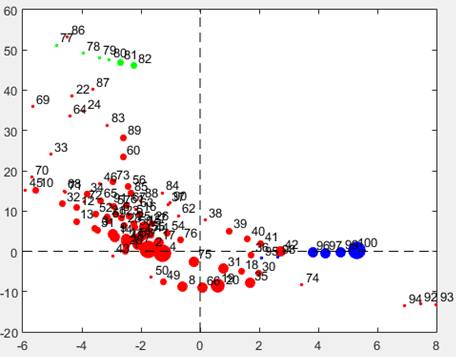
\includegraphics[width=0.8\textwidth]{imagenes/figuras/3_2.png}
\caption{Score plot en iterative y PLS.}
\end{figure}

\begin{figure}[H]
\centering
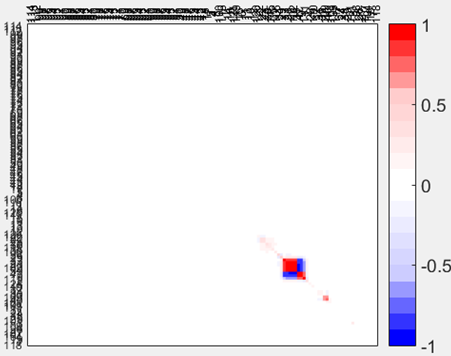
\includegraphics[width=0.8\textwidth]{imagenes/figuras/3_3.png}
\caption{MEDA en iterative y PLS.}
\end{figure}

\begin{figure}[H]
\centering
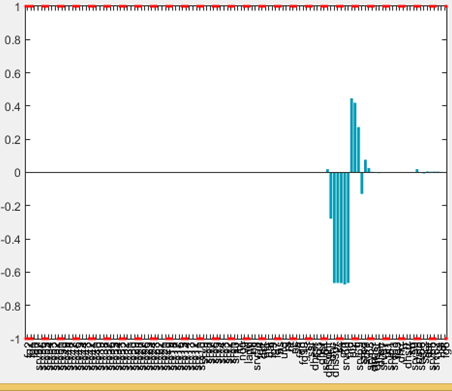
\includegraphics[width=0.8\textwidth]{imagenes/figuras/3_4.png}
\caption{oMEDA en iterative y PLS}
\end{figure}

\bigskip

Cuando se va a analizar conjuntos acotados de datos es más efectivo utilizar el “update” iterative, esto hace un preprocesamiento de los datos de todo el conjunto y después realiza el análisis, como es en el caso de los ejemplos de las figuras 3.2, 3.3 y 3.4. 
\bigskip

\begin{figure}[H]
\centering
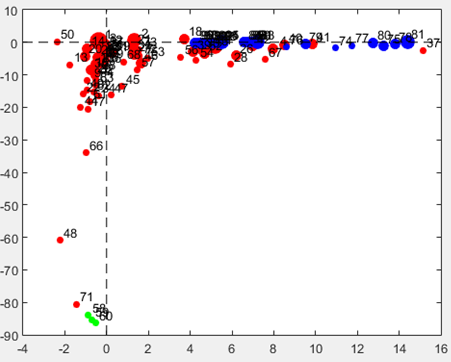
\includegraphics[width=0.8\textwidth]{imagenes/figuras/3_5.png}
\caption{Score plot en EWMA y PCA}
\end{figure}


\begin{figure}[H]
\centering
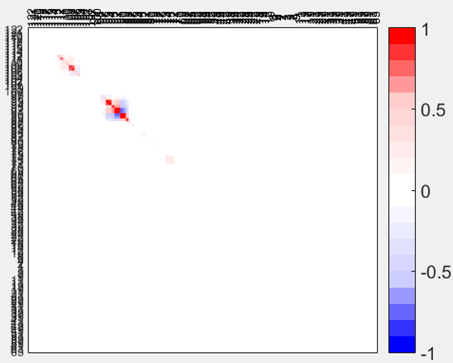
\includegraphics[width=0.8\textwidth]{imagenes/figuras/3_6.png}
\caption{MEDA en EWMA y PCA}
\end{figure}


\begin{figure}[H]
\centering
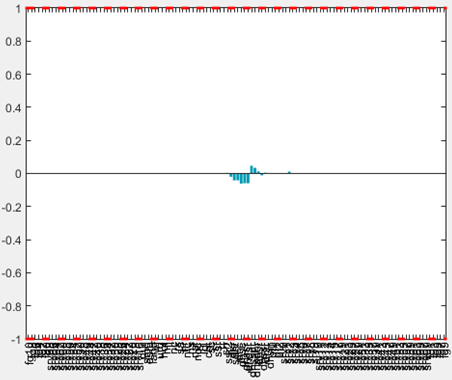
\includegraphics[width=0.8\textwidth]{imagenes/figuras/3_7.png}
\caption{oMEDA en EWMA y PCA}
\end{figure}


La estrategia EWMA utilizada en las figuras 3.5, 3.6, 3.7 se aplica para flujos constantes de datos, como streamings en los que continuamente se está recibiendo nueva información, por ello se usa un factor de olvido llamado en el caso del ejemplo de la Toolbox “lambda”, que va restando importancia a los datos conforme avanza el tiempo, para poder así analizar los nuevos que le van llegando.
\bigskip

Las diferencias que se dan entre las figuras con EWMA y con Iterative se dan por lo que se ha comentado anteriormente del preprocesamiento, EWMA en cada nuevo paquete de datos que le llega recalcula los valores de la media para incluir los nuevos en el análisis y mediante el factor de olvido los valores cambian de forma mas rápida.

\bigskip

Sin embargo en MEDA se puede observar como las figuras son muy similares, aunque en diferente posción, puesto que las relaciones entre variables se mantienen de forma continuada.
